\chapter{State of the Art} % Main chapter title

\label{Chapter3} % Change X to a consecutive number; for referencing this chapter elsewhere, use \ref{ChapterX}


\section{Introduction}

This chapter seeks to provide a comprehensive summary of the existing
approaches to tracking the face turns of a Rubik's Cube. The most
widely used solutions to date are found in Commercial Smartcubes
(\ref{sec:commercial-smartcubes}), but significant research has also
been carried out into Computer Vision based solutions
(\ref{subsec:computer-vision}). Other researchers have also explored
the use of magnetic resonance and a muscle-tracking armband
(\ref{sec:other-research})

This chapter will also explore a selection of wireless communication
techniques that at the time of writing have not been applied to the
challenge of tracking the moves of a Rubik's Cube. Specifically, this
chapter will review the potential usage of sound (\ref{subsec:sound}),
Radio Frequency Identification (RFID) (\ref{subsec:rfid}), and Off-Axis
Magnetic Angle Sensors (\ref{subsec:magnetic-angle-sensors}).

Finally, this chapter will close by detailing the specific research
questions this thesis will seek to answer
(\ref{sec:research-questions}).


\section{Commercial Smartcubes}
\label{sec:commercial-smartcubes}

Commercial Smartcubes are special Rubik's Cubes built around sensors
that can detect face turns and transmit that information over
Bluetooth. Some models can also measure and transmit data about the
cube's orientation.

At the time of writing, there are four major smartcubes on the market:
the Giiker Cube, the Go Cube, the Rubik's Connected (which is powered
by GoCube technology) and the Gans 356i. This section will discuss the
internal components of each of these cubes that provide this
move-tracking functionality.

\subsection{Giiker Cube}

The Xiaomi Giiker Cube was released in September 2018 making it the
first commercial smartcube on the market \cite{giiker-thecubicle}. This
"Supercube" as it was branded, used a relatively simple system for
tracking the cube's movements. The core of the cube is built around a
small circuit board with a microcontroller that measures the cube's
movements and a Bluetooth antenna that transmits those moves wirelessly
(Figure ~\ref{fig:giiker-internal-board}). The microcontroller detects
each face turn by reading the voltage drop across a small circuit
embedded within each center cap (Figure
~\ref{fig:giiker-center-front}). The center cap circuit controls its
output voltage by using a copper brush to change between four separate
electric paths, three different resistors and ground, as each face
rotates (Figure ~\ref{fig:giiker-center-brush}).
\cite{giiker-internals}

% How to do a sub-figure: https://tex.stackexchange.com/a/37597
\begin{figure}[h]
    \centering
    \caption{The internal components of the Giiker Cube}
    \label{fig:giiker-internal-components}
    \begin{subfigure}{0.25\textwidth}
        \centering
        \caption{Internal Board \cite{giiker-internals}}
        \label{fig:giiker-internal-board}
        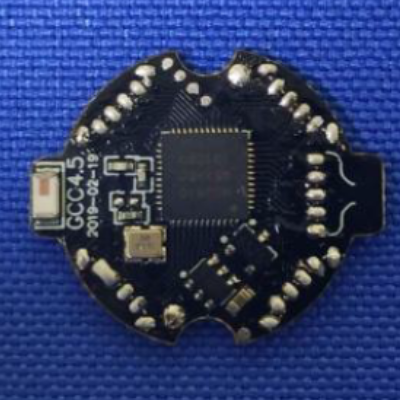
\includegraphics[width=.90\linewidth]{Figures/3 State of the Art/giiker-internal-board.png}
    \end{subfigure}%
    \begin{subfigure}{0.25\textwidth}
        \centering
        \caption{Center Cap Board \cite{eggins-giiker-internals}}
        \label{fig:giiker-center-front}
        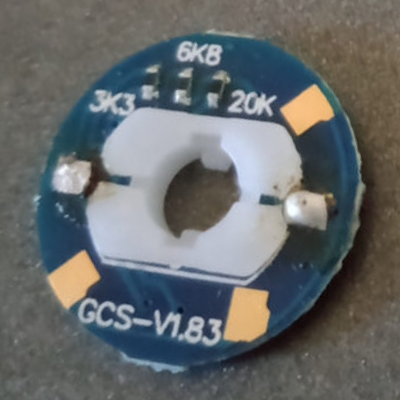
\includegraphics[width=.90\linewidth]{Figures/3 State of the Art/giiker-center-front.png}
    \end{subfigure}%
    \begin{subfigure}{0.25\textwidth}
        \centering
        \caption{Center Cap Pads \cite{eggins-giiker-internals}}
        \label{fig:giiker-center-pads}
        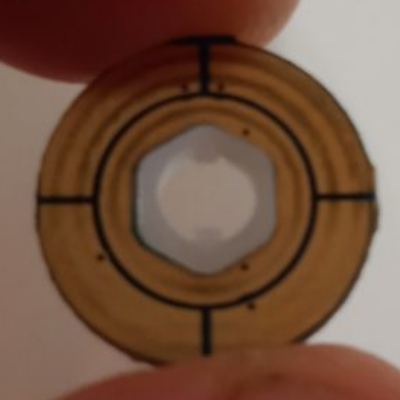
\includegraphics[width=.90\linewidth]{Figures/3 State of the Art/giiker-center-pads.png}
    \end{subfigure}%
    \begin{subfigure}{0.25\textwidth}
        \centering
        \caption{Center Cap Brush \cite{eggins-giiker-internals}}
        \label{fig:giiker-center-brush}
        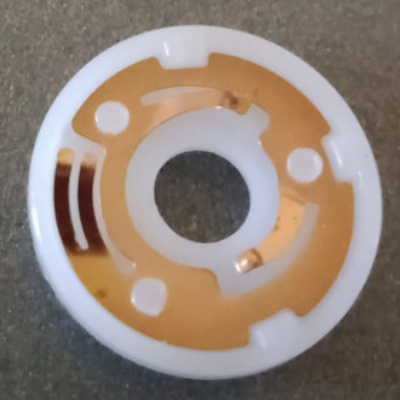
\includegraphics[width=.90\linewidth]{Figures/3 State of the Art/giiker-center-brush.png}
    \end{subfigure}%
\end{figure}

\subsection{Go Cube}

Announced on Kickstarter in June 2018, then shipped a year later
\cite{gocube-kickstarter}, Patricula's GoCube was the first smartcube
to include a gyroscope that would track a Rubik's Cube's orientation in
addition to the face turns applied to it.
\cite{gocube-product-launch-video} Like the Giiker Cube before it, the
GoCube's core contains a small circuit board with the main electronics
including a microcontroller, Bluetooth antenna, and the added gyroscope
(Figure ~\ref{fig:gocube-core}). Though the teardown pictures from the
Go Cube's FCC filing aren't particularly clear, it appears that the
cube registers face turns similarly to the Giiker Cube: by producing a
voltage drop via changing which one of the four resistors shown across
the bottom of the center cap board in Figure ~\ref{fig:gocube-cap-chip}
is in series with the circuit.

GoCube also serves as the underlying technology for the Rubik's Connected, the official smartcube from The Rubik's Company. \cite{gocube-rubiksconnected}

% How to do a sub-figure: https://tex.stackexchange.com/a/37597
\begin{figure}[h]
    \centering
    \caption{The internal components of the Go Cube \cite{gocube-internals}}
    \label{fig:gocube-internal-components}
    \begin{subfigure}{0.25\textwidth}
        \centering
        \caption{Internal Board}
        \label{fig:gocube-core}
        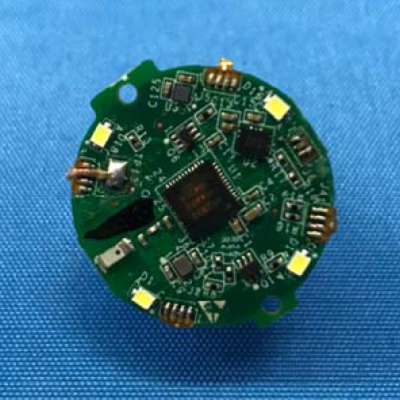
\includegraphics[width=.90\linewidth]{Figures/3 State of the Art/gocube-core.png}
    \end{subfigure}%
    \begin{subfigure}{0.25\textwidth}
        \centering
        \caption{Center Cap Board}
        \label{fig:gocube-cap-chip}
        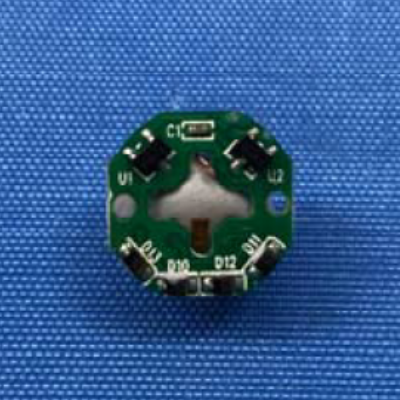
\includegraphics[width=.90\linewidth]{Figures/3 State of the Art/gocube-cap-chip.png}
    \end{subfigure}%
    \begin{subfigure}{0.50\textwidth}
        \centering
        \caption{Full Center Cap Teardown}
        \label{fig:gocube-centers}
        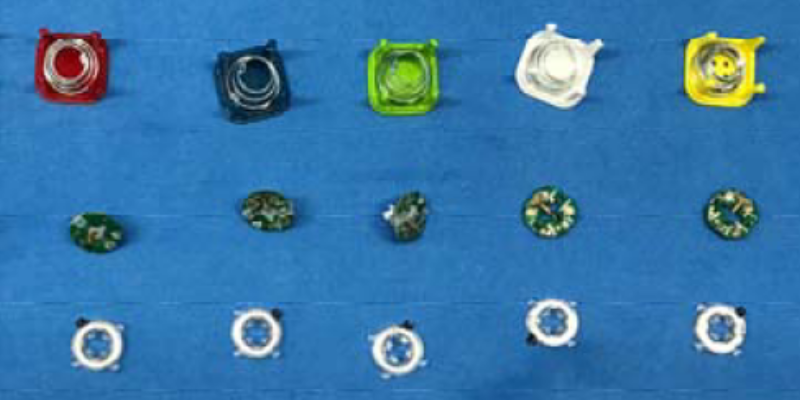
\includegraphics[width=.90\linewidth]{Figures/3 State of the Art/gocube-centers.png}
    \end{subfigure}%
\end{figure}

\subsection{Gans 356i}

Released in July 2019, the Gans 356i was the first commercial smartcube
produced by a traditional speedcube manufacturer.
\cite{gans356i-thecubicle} While the Gans 356i also uses a
microcontroller to process the face turns and Bluetooth to transmit the
move data, it tracks moves not through changing resistors in and out of
a circuit, but via six plastic rods that connect the outer center caps
to internal rotary encoders (Figure ~\ref{fig:gans356i-core}).

\begin{figure}[h]
    \centering
    \caption[Gans 356i Teardown]{The Gans 356i Cube's internal components. \cite{gans-356i-internals}}
    \label{fig:gans356i-core}
    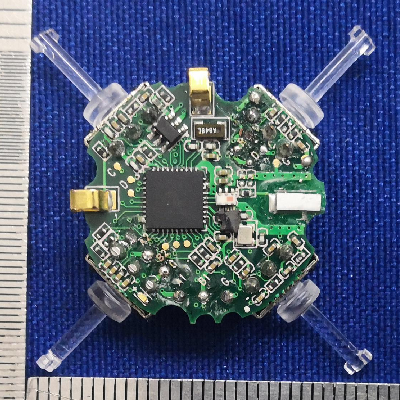
\includegraphics{Figures/3 State of the Art/gans356i-core.png}
\end{figure}


\section{Academia}
\label{sec:academia}

In addition to the various commercial smartcubes, many academic
research projects have involved some element of tracking the state/face
turns of a Rubik's Cube.

This section summarizes the current state of academic research into
using computer vision, magnetic resonance, and a muscle-tracking
armband to track the state of a Rubik's Cube.

\subsection{Computer Vision}
\label{subsec:computer-vision}

Computer Vision refers to the "field of Artificial Intelligence (AI)
that enables computers and systems to derive meaningful information
from digital images, videos, and other visual inputs."
\cite{ibm-cv-definition} Since human manipulation of a Rubik's Cube is
a physical, observable process, Computer Vision algorithms could be
developed to extract face turn information from videos of Rubik's Cube
solutions.

This section summarizes some of the relevant research in this area,
including computer vision algorithms capable of extracting individual
sticker colors from video, measuring the angle of rotation of a
specific face, and detection of entire face turns and face turn
sequences.

\subsubsection{Sticker Color Classification}

In 2015, Jay Hack, a graduate student studying Computer Science at
Stanford developed a neural network capable of recognizing the colors
of a Rubik's Cube face from video in various lighting conditions. His
algorithm could classify frames within 7 milliseconds with 92\%
accuracy. \cite{hackrubik}

\subsubsection{Measuring a Face's Angle of Rotation}

In 2019, OpenAI et al. published a viral video of a robot hand that had
taught itself to solve a Rubik's Cube. While the final, most successful
version of the robot hand's software used a Giiker Cube to obtain the
current rotational state of the cube, OpenAI et al. also researched the
viability of tracking a Rubik's Cube's position using only computer
vision. Their most successful vision-only algorithm measured only the
rotation angle of the top-most face on the Rubik's Cube and assumed
significant hardware requirements: a modified sticker set for the
Rubik's Cube, a well-lit environment, three strategically positioned
RBG Basler cameras, and a neural network trained on "a pool of
optimizer nodes, each of which uses 8 NVIDIA V100 GPUs and 64 CPU
cores". At peak performance, their vision-only algorithm's average
error (the difference between the predicted face angle and the actual
face angle) was 15.92$^\circ$, nearly three times the 5.90$^\circ$
average error of the hardware-based face angle measurement.
\cite{openai2019rubiks}

\subsubsection{Classification of Single Moves and Entire Move Sequences}

In 2020, Junshen Kevin Chen, Wanze Xie, and Zhouheng Sun, graduate
Computer Science students at Stanford created the DeepCube dataset
consisting of over 20,000 videos of Rubik's Cube face turns with
consistent lighting and backgrounds. They also built a neural network
to classify the videos with the face turn they contained. Their best
performing model only made "one mistake every 15 moves" which
corresponds to a 93.3\% accuracy. \cite{chendeepcube}


\subsection{Magnetic Resonance}

In 2018, Maria Mannone et al. used the IM3D magnetic 3D motion tracking
technology introduced by Huang et al. \cite{im3d} to track the state of
a Rubik's Cube across various movements for the purpose of generating a
sequence of musical chords. This approach to turn tracking requires a
special array of magnetic coils as shown in Figure
~\ref{fig:im3d-architecture} and the installation of "multiple small,
light-weight, wireless markers (LC coils) with unique IDs" (a process
that requires permanent modifications to the cube as evidenced by the
damaged plastic in Figure ~\ref{fig:cubeharmonic-trackers}). Mannone et
al. reported no issues with mistakes in this move tracking technology.
\cite{mannone-cubeharmonic-2018}

% How to do a sub-figure: https://tex.stackexchange.com/a/37597
\begin{figure}[h]
    \centering
    \caption{The IM3D technology as used in the Cube Harmonic}
    \label{fig:cubeharmonic-im3d}
    \begin{subfigure}{0.60\textwidth}
        \centering
        \caption{IM3D System Architecture \cite{im3d}}
        \label{fig:im3d-architecture}
        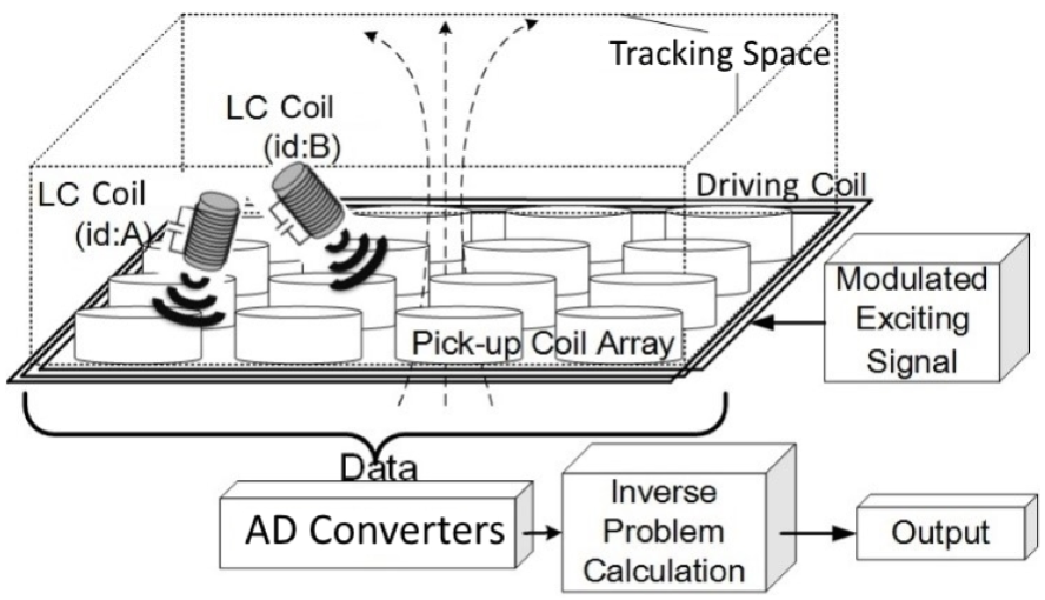
\includegraphics[width=.90\linewidth]{Figures/3 State of the Art/im3d.png}
    \end{subfigure}%
    \begin{subfigure}{0.40\textwidth}
        \centering
        \caption{IM3D trackers in a Rubik's Cube \cite{mannone-cubeharmonic-2019}}
        \label{fig:cubeharmonic-trackers}
        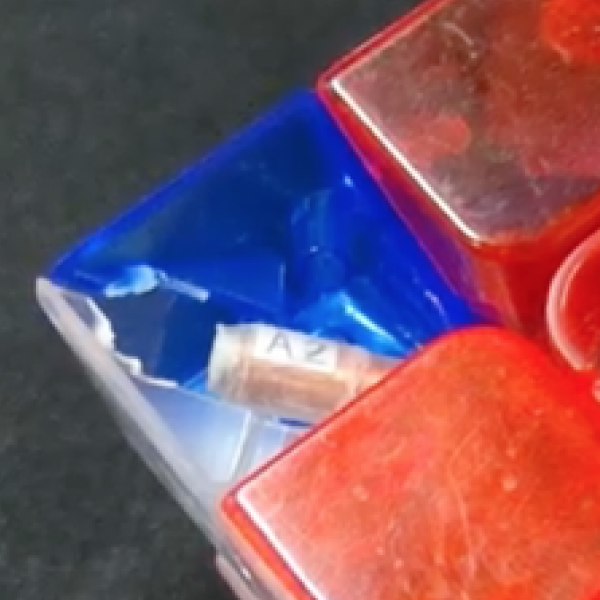
\includegraphics[width=.90\linewidth]{Figures/3 State of the Art/cubeharmonic-2019-tags.png}
    \end{subfigure}%
\end{figure}

\subsection{Muscle-Tracking Armband}

In 2017, Richard Polfreman and Benjamin Oliver researched ways to use
the face turns of a Rubik's Cube as controls for a music synthesizer.
They explored the use of a muscle-tracking armband (specifically the
Myo Armband) to track the human solver's finger movements while
manipulating the cube. However, since "the Myo moved a little when
'cubing'", they ultimately found greater success with a computer vision
based tracking solution similar to those discussed in
\ref{subsec:computer-vision}. \cite{polfreman-musiccube}


\section{Other Relevant Research}
\label{sec:other-research}

Finally, there are a number of research papers/commercial products that
seek to transmit data in highly-constrained environments that are
potentially relevant to the challenge of tracking the turns of a
Rubik's Cube.

This section discusses some of these potential alternate move tracking
mediums, specifically sound, RFID, and off-angle magnetic rotation
sensors.

\subsection{Sound}
\label{subsec:sound}

Sound is another communication medium that could be leveraged to track
the moves of a Rubik's Cube. In 2015, Jonas Michel, a researcher at The
University of Texas at Austin documented his exploration of the
viability of creating an "acoustic modem" to transmit an arbitrary
sequence of bits using sound. He observed that "as commercial
off-the-shelf (COTS) smartphones become more powerful, it is worthwhile
to revisit the use of sound as a medium for aerial digital
device-to-device communications." \cite{michel-sound}

Indeed, since many speedcubers practice by timing solves on a
microphone-equipped smartphone or laptop\footnote{One of the highest
rated cubing timers on Android, Twisty Timer, has over 100,000
downloads on the Google Play Store \cite{googleplay-twistytimer}. By
comparison, SpeedSolving.com, the central forum for speedcubing related
discussion, has about 43,000 members \cite{speedsolving-com}}, sound is
a promising alternative communication medium to existing
Bluetooth-based smartcubes.

\subsection{Radio Frequency Identification (RFID)}
\label{subsec:rfid}

Radio Frequency Identification (RFID) is a wireless technology often
used in supply-chain systems \cite{rfid-rotary-encoder} based on
individual tags that can transmit a fixed set of information to a
nearby reader. \cite{fda-rfid}. In 2018, Genovesi et al. proposed a
rotary encoder based on RFID that produced angle measurements accurate
to within 3$^\circ$ after a calibration that "must only be done once
(when the sensor is put in place) if the distance between the reader
and the tag does not change." \cite{rfid-rotary-encoder}

While this approach may not be particularly useful for tracking the
moves of human speedcubers since their movement of the cube would
require constant re-calibration, it could be used in robotics based
applications desiring to track the ongoing state of the cube.

\subsection{Off-Axis Magnetic Angle Sensors}
\label{subsec:magnetic-angle-sensors}

Another unique type of rotary encoder is an off-angle magnetic
rotational sensor like the ones produced by NVE Corporation.
\cite{nve-mag-sensor} In the context of a Rubik's Cube, a properly
sized diametric ring magnet could be fastened to the inner screw below
the center cap of each face of the cube and the resulting optimal
position for the magnetic sensor would stay within the walls of the
center cap as shown by the the $z_0$ and $R_0$ values in Figure
~\ref{fig:nve-mag-calculations} which are smaller than the 8 mm
distance between the center screw and the inner wall of the center cap
in a standard-sized cube like the Gans 356.

\begin{figure}[h]
    \centering
    \caption[Off-Angle Magnetic Sensor Calculations]{Off-Angle Magnetic Sensor Calculations \cite{nve-mag-sensor-calculations}}
    \label{fig:nve-mag-calculations}
    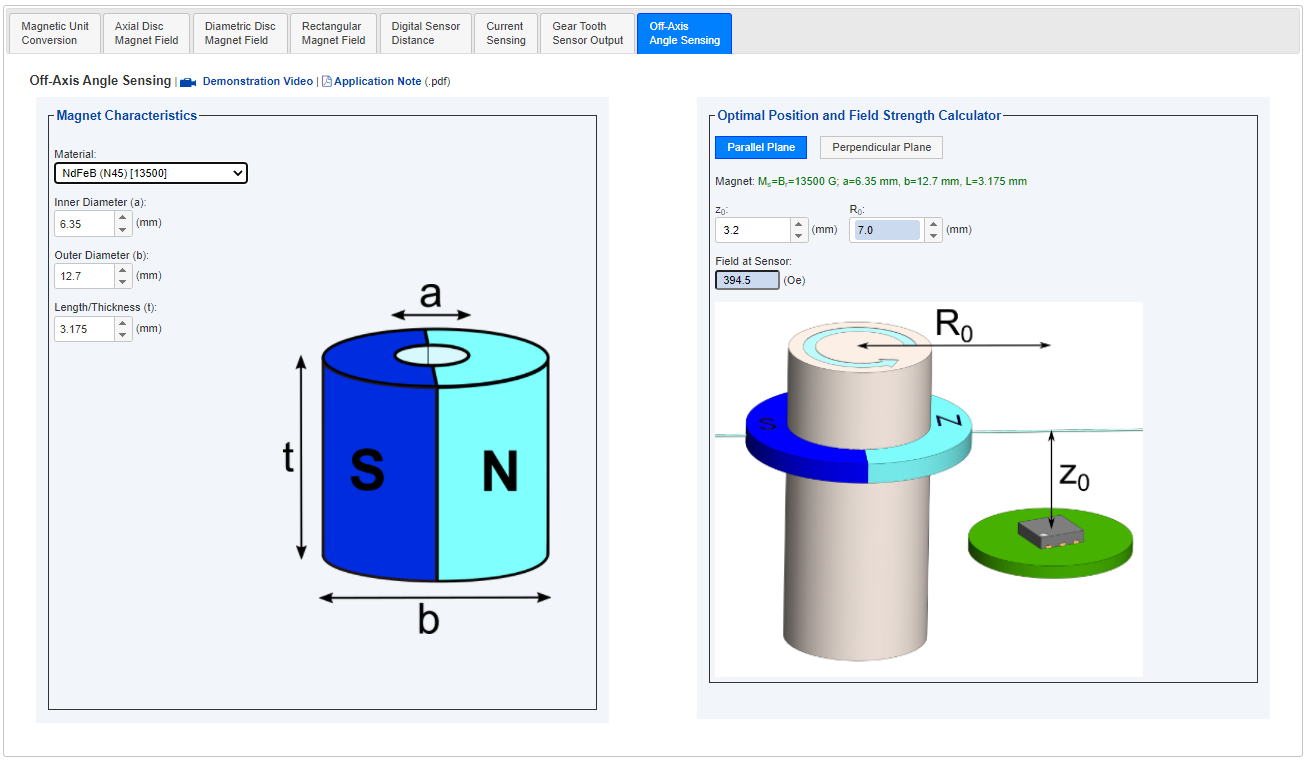
\includegraphics[width=\linewidth]{Figures/3 State of the Art/nve-mag-calculations.png}
\end{figure}


\section{Research Questions}
\label{sec:research-questions}

While there are many effective solutions for tracking the moves of a
Rubik's Cube if the cube is built for that purpose, there does not yet
exist a comparably effective technique for tracking the moves of a
standard, "non-smart" Rubik's Cube. As shown above, significant effort
has been spent researching and developing solutions that can leverage
the Bluetooth transmitters and camera sensors of consumer grade
smartphones and laptops with varying degrees of success. However,
little to no research has been carried out exploring the viability of
using the microphones readily available on the same devices for this
purpose.

Thus, this thesis will seek to answer the overarching question from
Chapter \ref{Chapter1} \emph{"Is it possible to track the face turns of
a standard, "non-smart" speedcube in a non-destructive,
competition-legal way?"} by detailing a proof-of-concept for a
sound-based smartcube design created in response to the following
questions:

\begin{enumerate}

    \item \textbf{Feasibility on Consumer Hardware}: \emph{What are the
    constraints for a sound-based smartcube design compatible with
    consumer-grade microphones like those found in common smartphones
    and laptops?}
    
    \item \textbf{Move Tracking Accuracy}: \emph{How could such a
    sound-based smartcube design track the face turns of a Rubik's
    Cube with high accuracy?}
    
    \item \textbf{Compatibility with Standard Speedcubes}: \emph{How
    could such a sound-based smartcube design be deployed within a
    standard, "non-smart" speedcube without requiring permanent
    modifications to the original cube?}

    \item \textbf{Move Tracking Granularity}: \emph{How could such a
    sound-based smartcube design record the time spent executing each
    individual face turn of a Rubik's Cube?}
    
    \item \textbf{Competition Legality}: \emph{How could such a
    sound-based smartcube design comply with competition regulations
    prohibiting the use of electronics while performing a competitive
    solve?}
    
\end{enumerate}
